\chapter{Diagramas de secuencia}
\label{chap:anexo2}

En esta sección vamos a especificar cómo opera el sistema ante las acciones del actor mediante diagramas de secuencia del sistema. 

\subsection{Apertura y cierra de sesión}

\subsubsection{Inicio de sesión}

\begin{figure}[H]
	\centering
	\includegraphics[width=1\textwidth]{imagenes/imagenesDiagramas/InicioCierre/inicioSesión.jpg}
	\caption{Diagrama de secuencia de inicio de sesión}
	\label{fig:seqdiag1}
\end{figure}

\subsubsection{Cierre de sesión}

\begin{figure}[H]
	\centering
	\includegraphics[width=1\textwidth]{imagenes/imagenesDiagramas/InicioCierre/cierreSesión.jpg}
	\caption{Diagrama de secuencia de cierre de sesión}
	\label{fig:seqdiag2}
\end{figure}

\subsection{Gestión de artículos}

\subsubsection{Introducción de un nuevo artículo}

\begin{figure}[H]
	\centering
	\includegraphics[width=1\textwidth]{imagenes/imagenesDiagramas/Articulos/nuevoArtículo.jpg}
	\caption{Diagrama de secuencia de un nuevo artículo}
	\label{fig:seqdiag3}
\end{figure}

\subsubsection{Edición de un artículo existente}

\begin{figure}[H]
	\centering
	\includegraphics[width=1\textwidth]{imagenes/imagenesDiagramas/Articulos/editarArtículo.jpg}
	\caption{Diagrama de secuencia de edición de un artículo}
	\label{fig:seqdiag4}
\end{figure}

\subsubsection{Eliminación de un artículo}

\begin{figure}[H]
	\centering
	\includegraphics[width=1\textwidth]{imagenes/imagenesDiagramas/Articulos/eliminarArtículo.jpg}
	\caption{Diagrama de secuencia de eliminación de un artículo}
	\label{fig:seqdiag5}
\end{figure}

\subsubsection{Visualización de los datos de un artículo}

\begin{figure}[H]
	\centering
	\includegraphics[width=1\textwidth]{imagenes/imagenesDiagramas/Articulos/visualizarDatosArtículo.jpg}
	\caption{Diagrama de secuencia de visualización de datos de un artículo}
	\label{fig:seqdiag6}
\end{figure}

\subsubsection{Búsqueda de un artículo por nombre}

\begin{figure}[H]
	\centering
	\includegraphics[width=1\textwidth]{imagenes/imagenesDiagramas/Articulos/buscarArtículo.jpg}
	\caption{Diagrama de secuencia de búsqueda de un artículo}
	\label{fig:seqdiag7}
\end{figure}

\subsubsection{Categorización de un artículo}

\begin{figure}[H]
	\centering
	\includegraphics[width=1\textwidth]{imagenes/imagenesDiagramas/Articulos/categorizarArtículos.jpg}
	\caption{Diagrama de secuencia de categorización de un artículo}
	\label{fig:seqdiag8}
\end{figure}

\subsubsection{Visualización de la lista de artículos}

\begin{figure}[H]
	\centering
	\includegraphics[width=1\textwidth]{imagenes/imagenesDiagramas/Articulos/visualizarListaArtículos.jpg}
	\caption{Diagrama de secuencia de visualización de la lista de artículos}
	\label{fig:seqdiag9}
\end{figure}

\subsection{Gestión de inventario}

\subsubsection{Actualización del inventario de forma automática}

\begin{figure}[H]
	\centering
	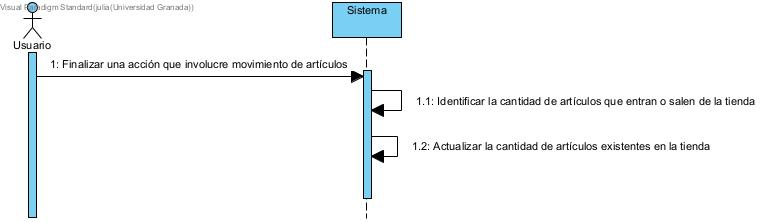
\includegraphics[width=1\textwidth]{imagenes/imagenesDiagramas/Articulos/actualizarInventario.jpg}
	\caption{Diagrama de secuencia de actualización de inventario}
	\label{fig:seqdiag10}
\end{figure}

\subsubsection{Visualización de la lista de renovación de artículos}

\begin{figure}[H]
	\centering
	\includegraphics[width=1\textwidth]{imagenes/imagenesDiagramas/Articulos/visualizarListaRenovación.jpg}
	\caption{Diagrama de secuencia de visualización de la lista de renovación de artículos}
	\label{fig:seqdiag11}
\end{figure}

\subsection{Gestión de clientes}

\subsubsection{Registro de un nuevo cliente habitual}

\begin{figure}[H]
	\centering
	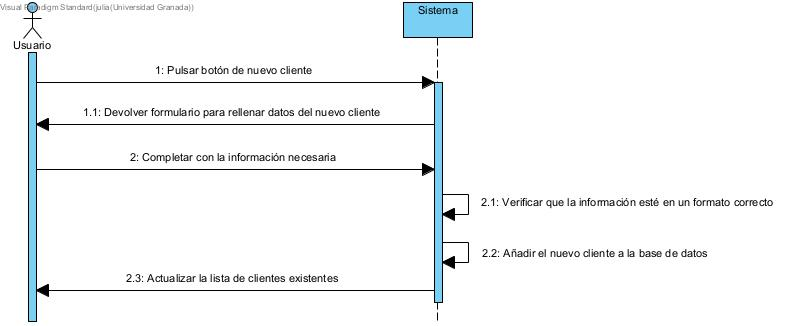
\includegraphics[width=1\textwidth]{imagenes/imagenesDiagramas/Cliente/nuevoCliente.jpg}
	\caption{Diagrama de secuencia de registro de un cliente}
	\label{fig:seqdiag12}
\end{figure}

\subsubsection{Edición de los datos de un cliente existente}

\begin{figure}[H]
	\centering
	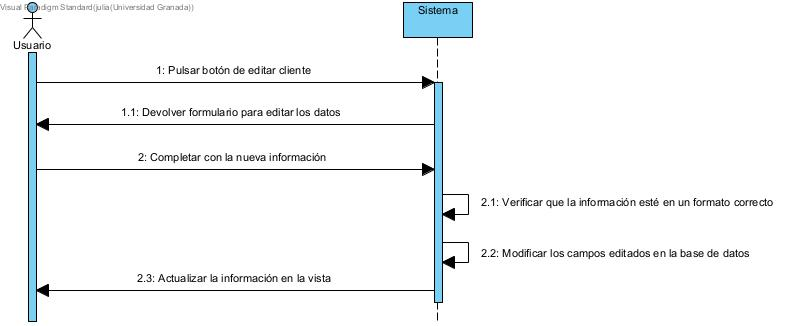
\includegraphics[width=1\textwidth]{imagenes/imagenesDiagramas/Cliente/editarCliente.jpg}
	\caption{Diagrama de secuencia de edición de los datos de un cliente}
	\label{fig:seqdiag13}
\end{figure}

\subsubsection{Eliminación de un cliente existente}

\begin{figure}[H]
	\centering
	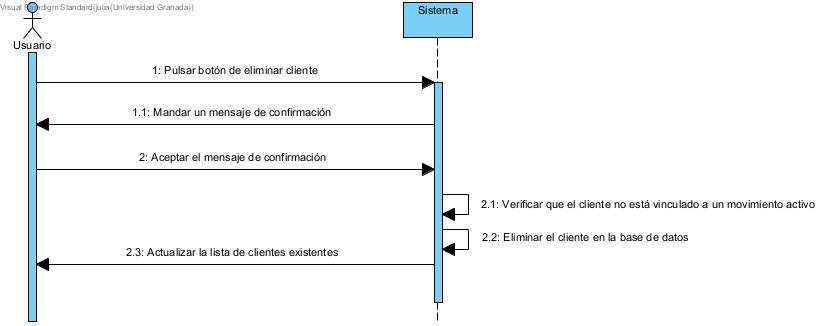
\includegraphics[width=1\textwidth]{imagenes/imagenesDiagramas/Cliente/eliminarCliente.jpg}
	\caption{Diagrama de secuencia de eliminación de un cliente}
	\label{fig:seqdiag14}
\end{figure}

\subsubsection{Visualización de los datos de un cliente}

\begin{figure}[H]
	\centering
	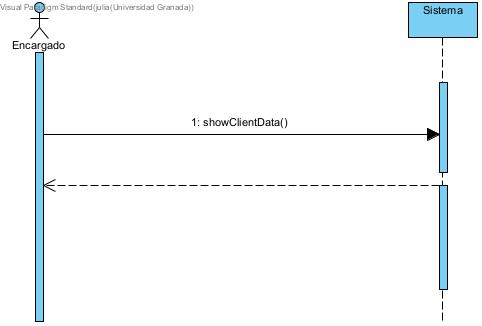
\includegraphics[width=1\textwidth]{imagenes/imagenesDiagramas/Cliente/visualizarDatosCliente.jpg}
	\caption{Diagrama de secuencia de visualización de los datos de un cliente}
	\label{fig:seqdiag15}
\end{figure}

\subsubsection{Visualización la lista de clientes existentes}

\begin{figure}[H]
	\centering
	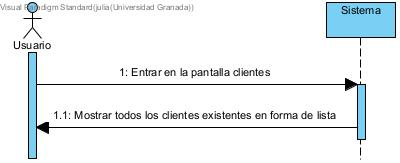
\includegraphics[width=1\textwidth]{imagenes/imagenesDiagramas/Cliente/visualizarListaClientes.jpg}
	\caption{Diagrama de secuencia de visualización de la lista de clientes}
	\label{fig:seqdiag16}
\end{figure}

\subsubsection{Búsqueda de un cliente por nombre}

\begin{figure}[H]
	\centering
	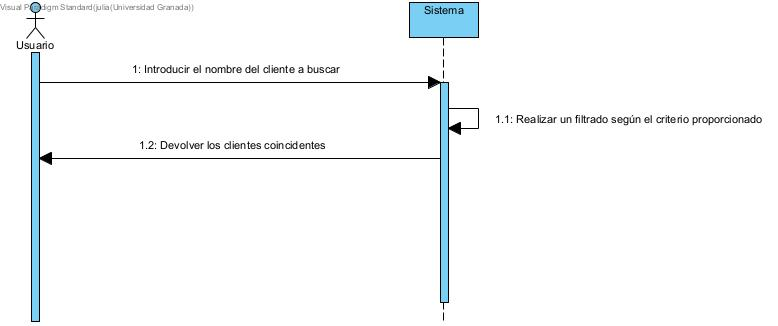
\includegraphics[width=1\textwidth]{imagenes/imagenesDiagramas/Cliente/buscarClientes.jpg}
	\caption{Diagrama de secuencia de búsqueda de un cliente}
	\label{fig:seqdiag17}
\end{figure}

\subsubsection{Filtrado de clientes con préstamos}

\begin{figure}[H]
	\centering
	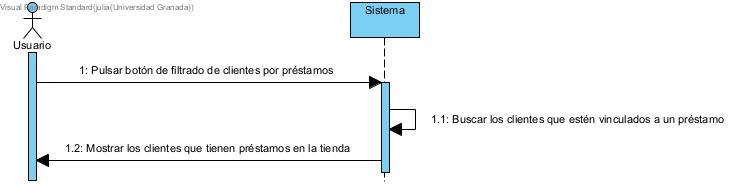
\includegraphics[width=1\textwidth]{imagenes/imagenesDiagramas/Cliente/filtrarClientes.jpg}
	\caption{Diagrama de secuencia de filtrado de clientes}
	\label{fig:seqdiag18}
\end{figure}

\subsection{Gestión de movimientos}

\subsubsection{Introducción de una nueva venta}

\begin{figure}[H]
	\centering
	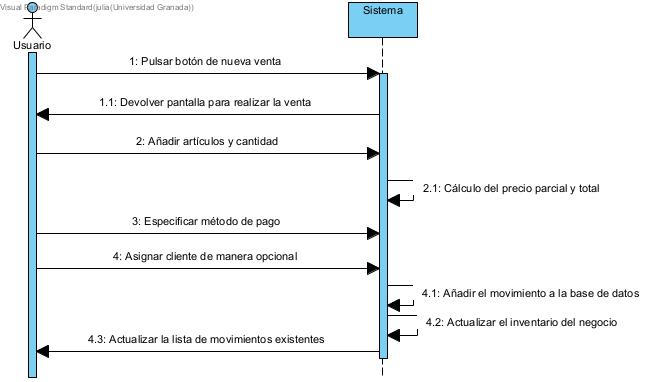
\includegraphics[width=1\textwidth]{imagenes/imagenesDiagramas/Movimientos/nuevaVenta.jpg}
	\caption{Diagrama de secuencia de nueva venta}
	\label{fig:seqdiag19}
\end{figure}

\subsubsection{Introducción de un nuevo préstamo}

\begin{figure}[H]
	\centering
	\includegraphics[width=1\textwidth]{imagenes/imagenesDiagramas/Movimientos/nuevoPréstamo.jpg}
	\caption{Diagrama de secuencia de nuevo préstamo}
	\label{fig:seqdiag20}
\end{figure}

\subsubsection{Introducción de una nueva devolución}

\begin{figure}[H]
	\centering
	\includegraphics[width=1\textwidth]{imagenes/imagenesDiagramas/Movimientos/realizarDevolución.jpg}
	\caption{Diagrama de secuencia de nueva devolución}
	\label{fig:seqdiag21}
\end{figure}

\subsubsection{Eliminación de un movimiento}

\begin{figure}[H]
	\centering
	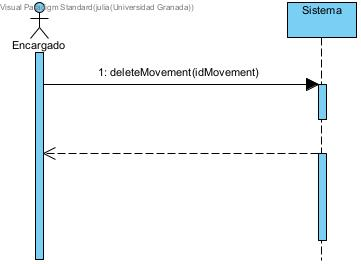
\includegraphics[width=1\textwidth]{imagenes/imagenesDiagramas/Movimientos/eliminarMovimiento.jpg}
	\caption{Diagrama de secuencia de eliminación de un movimiento}
	\label{fig:seqdiag22}
\end{figure}

\subsubsection{Visualización de los datos de un movimiento}

\begin{figure}[H]
	\centering
	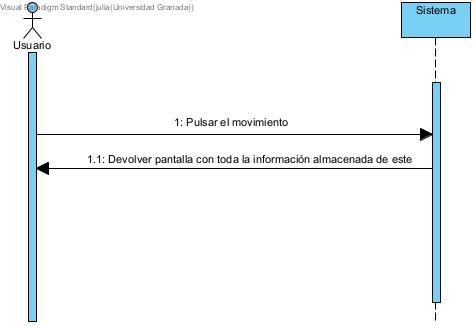
\includegraphics[width=1\textwidth]{imagenes/imagenesDiagramas/Movimientos/visualizarDatosMovimiento.jpg}
	\caption{Diagrama de secuencia de visualización de datos de un movimiento}
	\label{fig:seqdiag23}
\end{figure}

\subsubsection{Visualización de la lista de movimientos existentes}

\begin{figure}[H]
	\centering
	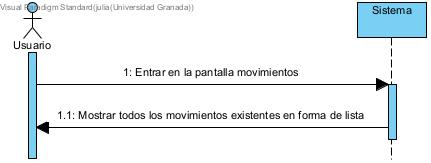
\includegraphics[width=1\textwidth]{imagenes/imagenesDiagramas/Movimientos/visualizarListaMovimientos.jpg}
	\caption{Diagrama de secuencia de visualización la lista de movimientos}
	\label{fig:seqdiag24}
\end{figure}

\subsubsection{Filtrado de los movimientos según su tipo}

\begin{figure}[H]
	\centering
	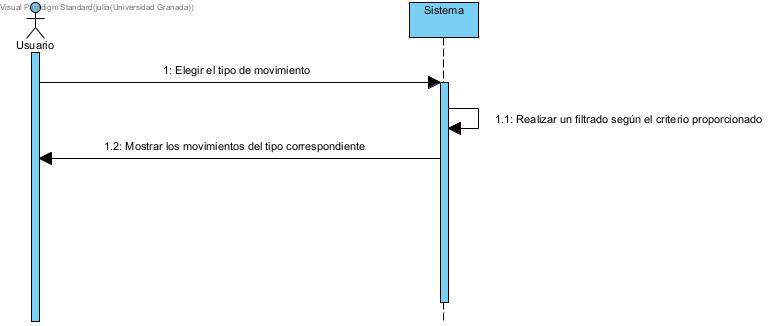
\includegraphics[width=1\textwidth]{imagenes/imagenesDiagramas/Movimientos/filtrarMovimientos.jpg}
	\caption{Diagrama de secuencia del filtrado de movimientos}
	\label{fig:seqdiag25}
\end{figure}

\subsubsection{Búsqueda de movimientos por fecha o cliente}

\begin{figure}[H]
	\centering
	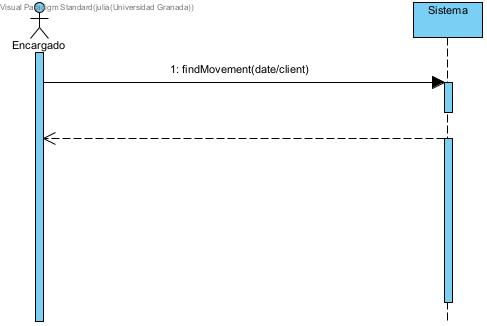
\includegraphics[width=1\textwidth]{imagenes/imagenesDiagramas/Movimientos/buscarMovimientos.jpg}
	\caption{Diagrama de secuencia de búsqueda de movimientos}
	\label{fig:seqdiag26}
\end{figure}

\subsubsection{Generación de una compra a partir de un préstamo}

\begin{figure}[H]
	\centering
	\includegraphics[width=1\textwidth]{imagenes/imagenesDiagramas/Movimientos/compraDesdePréstamo.jpg}
	\caption{Diagrama de secuencia de generación de una compra desde un préstamo}
	\label{fig:seqdiag27}
\end{figure}

\subsection{Gestión de resúmenes y gráficas}

\subsubsection{Visualización de la caja diaria}

\begin{figure}[H]
	\centering
	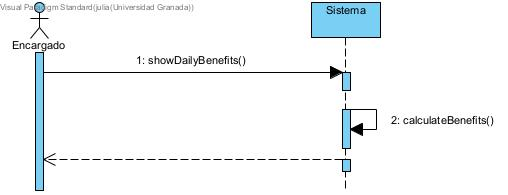
\includegraphics[width=1\textwidth]{imagenes/imagenesDiagramas/Graficos/visualizarCajaDiaria.jpg}
	\caption{Diagrama de secuencia de visualización de la caja diaria}
	\label{fig:seqdiag28}
\end{figure}

\subsubsection{Visualización de gráficos}

\begin{figure}[H]
	\centering
	\includegraphics[width=1\textwidth]{imagenes/imagenesDiagramas/Graficos/visualizarGráficos.jpg}
	\caption{Diagrama de secuencia de visualización de gráficos}
	\label{fig:seqdiag29}
\end{figure}

